\section{Application of the EAMPA Code}


\subsection[Potential Transferability]{Investigating the Transferability of Existing Potentials}

There are currently a number of \acrshort{eam} Iron potentials, as well as a \acrshort{meam} potential for Fe-Pd.  Several pure element potentials also exist for Ruthenium and Palladium.  Whilst it would be convenient to have a one size fits all potential, this is not the case.  Taking the Ruthenium potential as an example, in work that required the reproduction of stacking fault and surface energy of the element, the existing potentials were inadequate and a new potential was developed\cite{mendelevruau}.

Several potentials were selected to test transferability.  First, the FCC Sheng potential for Aluminium was applied to both FCC and BCC structures in the EAMPA code.  The properties of FCC Aluminium are known, and those for BCC Aluminium were calculated using DFT.  This investigation shows that some properties, such as the lattice constant, does transfer quite well to the new structure, but the bulk modulus and $C_{11}$ elastic constant are both poorly reproduced (table \ref{table:alshengtransferability}).  

\begin{table}[h]
\begin{center}
\begin{tabular}{c c c c c}
\hline\hline
Property   & Al FCC Exp. & Al FCC Sheng &  Al BCC DFT & Al BCC Sheng \\
\hline\hline
a0             & 4.05  &  4.02        & 3.23     & 3.18     \\
e0             & -3.36 & -3.36        & -3.26    & -3.27    \\
b0             & 76    &  86          & 69       & 50       \\
$C_{11}$       & 114   &  124 (125)   & 47 (47)  & 11 (5)   \\
$C_{12}$       & 62    &  67 (66)     & 81 (24)  & 70 (63)  \\
$C_{44}$       & 32    &  29 (32)     & 40 (12)  & 29 (42)  \\
\hline\hline
\end{tabular}
\end{center}
\caption{Applying the Sheng Al potential, developed for FCC crystals, to the BCC structure.  Elastic constants are calculated using the method by Mehl et al with values from the method by Ravindran et al in brackets.}
\label{table:alshengtransferability}
\end{table}

The Mendelev 2003 potential was developed to fit the properties of BCC Iron, but also to reproduce the transition from BCC to FCC at high temperatures.  However, when using this potential for low  temperature FCC Iron, it does not reproduce the properties predicted by DFT.  All 9 orthorhombic elastic constants have been omitted in table \ref{table:femendelevtransferability}, but there is a significant difference for the three elastic constants given as well as the bulk modulus.

\begin{table}[h]
\begin{center}
\begin{tabular}{c c c c c}
\hline\hline
Property   & Fe BCC Exp. & Fe BCC Mendelev &  Fe FCC DFT & Fe FCC Mendelev \\
\hline\hline
a0             &   2.86  &   2.86      &   3.42   &   3.59          \\
e0             &  -4.32  &  -4.13      &  -4.26   &  -4.01          \\
b0             &   170  &    176       &  226     &   98            \\
$C_{11}$       &   243  &   255 (260)  &  364     &   6 (79)        \\
$C_{12}$       &   145  &   137 (143)  &  142     &   145 (69)      \\
$C_{44}$       &   116  &   114 (111)  &  186     &   86 (48)       \\
\hline\hline
\end{tabular}
\end{center}
\caption{Applying the Sheng Al potential, developed for FCC crystals, to the BCC structure.  Elastic constants are calculated using the method by Mehl et al with values from the method by Ravindran et al in brackets.}
\label{table:femendelevtransferability}
\end{table}

Finally the Ackland 1997 potential for Iron was tested.  This older potential gives a better value for the cohesive energy when transferred to the FCC structure, but other properties such as the relaxed lattice constant are quite different (table \ref{table:feacklandtransferability}).

\begin{table}[h]
\begin{center}
\begin{tabular}{c c c c c}
\hline\hline
Property   & Fe BCC Exp. & Fe BCC Mendelev &  Fe FCC DFT & Fe FCC Mendelev \\
\hline\hline
a0             &   2.86  &   2.87      &   3.42   &   3.62          \\
e0             &  -4.32  &  -4.32      &  -4.26   &  -4.26          \\
b0             &   170  &    200       &  226     &   141            \\
$C_{11}$       &   243  &   265 (248)  &  364     &   117 (140)        \\
$C_{12}$       &   145  &   168 (151)  &  142     &   153 (117)      \\
$C_{44}$       &   116  &   125 (128)  &  186     &   164 (94)       \\
\hline\hline
\end{tabular}
\end{center}
\caption{Applying the Sheng Al potential, developed for FCC crystals, to the BCC structure.  Elastic constants are calculated using the method by Mehl et al with values from the method by Ravindran et al in brackets.}
\label{table:feacklandtransferability}
\end{table}

This investigation into existing potentials shows that whilst some of the properties are replicated, many do not match the DFT computed values.  This supports the derivation of new potentials to be fit that replicate the DFT values and take into account the characteristics of a number of provided configurations.  Additional plots are included in the appendix that show the expected equations of state compared to those generated using the above potentials (section \ref{section:transferabilityappendix}).




\subsection{Fitting Potentials with EAMPA}

The fitting process was computationally intensive and utilised nodes on the University of Birmingham BlueBEAR computer.  At the time of writing, the code was able to fit energy, forces and bulk properties.  I was not convinced that the computation of stress in EAMPA and in PWscf were identical and so throughout I set the weighting of stress to zero.

\subsection{Choice of Function and Functional}

A number of functions and functionals have been used previously and these are discussed in detail in chapter \ref{chap:backgroundfitting}.  Several were used to attempt to fit the potentials, but eventually the cubic splines and tight binding type functional, as used by Mendelev, Ackland, Bonny et al, were selected.

Initially, I looked to the computer program DIRAC for the density function, as it computes the radial electron density distribution (figure \ref{fig:dirac-fe-density-plot} and figure \ref{fig:dirac-fe-density-plot}).  Unfortunately, as may be expected, there were a number of issues in using the density distribution of a single atom.  The atomic separation for both iron and palladium, for a relaxed crystal, begins at approximately 2-2.5 angstrom, but most of the electrons, from all shells, are distributed much closer.  The plot does not take into consideration the valence electrons shared in the crystal, bonding the metal atoms together.

From the point of view of the potential, the pair potential will dominate at small separations due to the \acrshort{zbl} function.  The density function will be important at separations of 2 angstrom up to the cutoff radius (5-6 angstrom).  For this reason, the idea to use the DIRAC computed densities was abandoned in favour of a cubic spline.

\begin{figure}[htb]
\minipage{0.49\textwidth}
	\begin{center}
  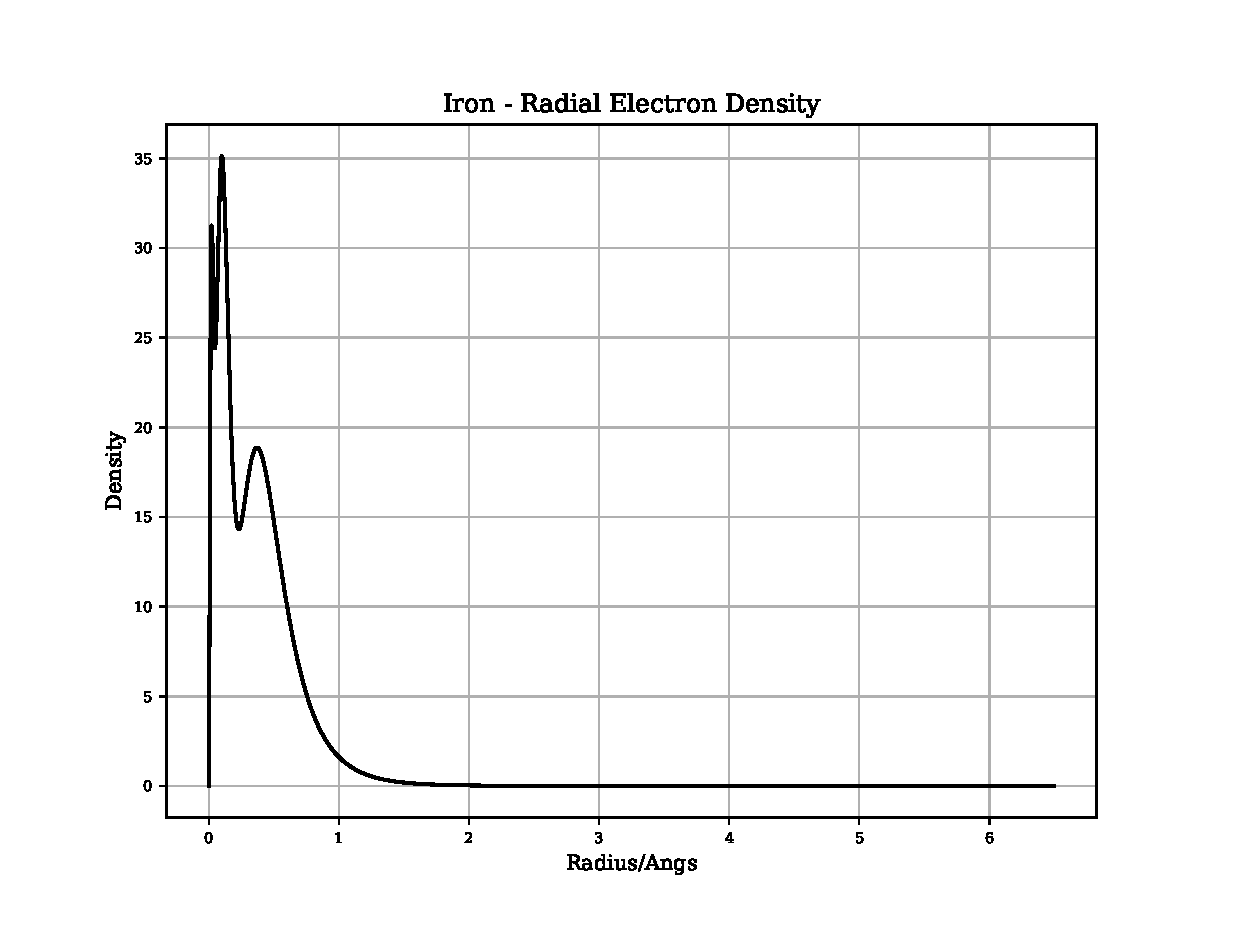
\includegraphics[width=0.9\linewidth]{chapters/potentials_fe_pd_ru/density/fe.eps}
  \captionsetup{font={it}}
  \caption{DIRAC calculated radial electron density for Iron}
  \label{fig:dirac-fe-density-plot}
	\end{center}
\endminipage\hfill
\minipage{0.49\textwidth}
	\begin{center}
  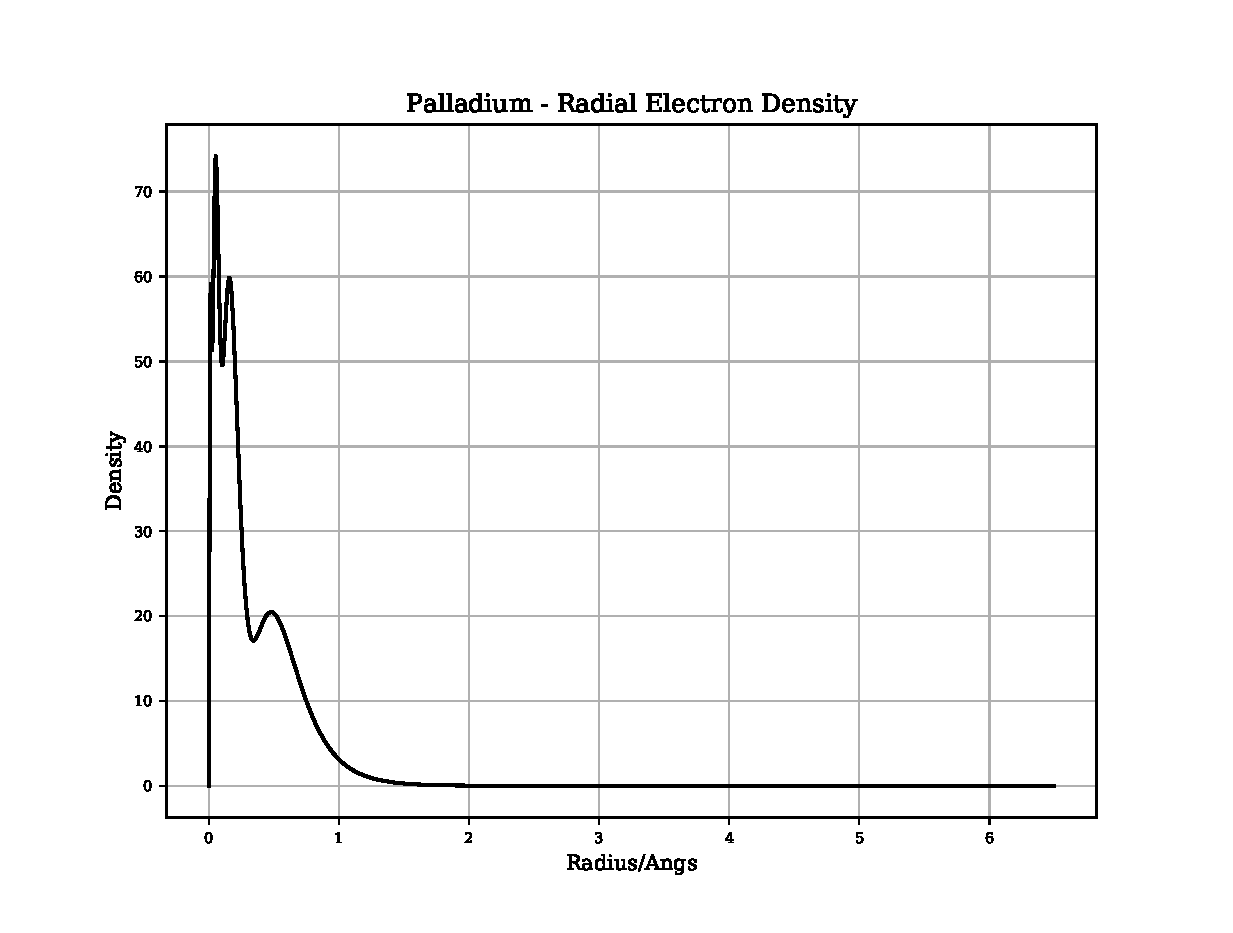
\includegraphics[width=0.9\linewidth]{chapters/potentials_fe_pd_ru/density/pd.eps}
  \captionsetup{font={it}}
  \caption{DIRAC calculated radial electron density for Palladium}
  \label{fig:dirac-pd-density-plot}
	\end{center}
\endminipage
\end{figure}

One interesting feature that Bonny used in his code was to add a hard core spline to the pair potential with a positive coefficient.  This was to ensure that at small separations, say below 1.5-1.8 angstrom, the atoms would repel.  The cubic spline used in this work for the density also has a fixed positive coefficient to help stop negative densities for small separations.  This is dependent on the number of cubic splines used, and is a feature that can be turned off in the EAMPA code.

A cubic spline was also used for the pair potential, and as with Bonny's code, this had a hard core potential but in addition to this a \acrshort{zbl} core was added to the entire potential to ensure the exponential increase in energy as modelled with the \acrshort{zbl} function.  This was to ensure the potential would both model the material when out of a radiation field, where the atoms are several angstrom apart, but also able to capture a damage cascade where the separation drops and the \acrshort{zbl} becomes the dominant feature, over both the pair cubic spline and the embedding functional.

There was a choice of several embedding functionals but one based on the Finnis-Sinclair and \acrshort{eam} was used.  It consisted of the square root term but also a zeroth power and square term for greater flexibility.  The addition of a fourth power term had been trailed, but occasionally when fitting the parameters the coefficient of the fourth power would become negative leading to a negative energy at high electron densities.


\subsection{Searching Parameter Space}

Improving the potential was an iterative process that required multiple runs of EAMPA feeding the last potential as a starting point for the next potential.  In the first instance, the exact bulk property fitting code of Bonny was used, but it did not always find the parameters that reproduced the data points it was given.  This was perhaps due to a lack of data and knowledge on how to use the code effectively, but it did give a starting point with a modest number of cubic splines for the density and pair functions.

These initial set of parameters were then used with EAMPA.  The first task with this code was to find parameters that replicated the energies, forces and bulk properties for each of the pure elements.

The type of search could be adjusted for each fitting job, but the typical process was as follows.  A short random search through parameter space followed by a small simulated annealing search with a wide search area.  This was then followed by a genetic algorithm search with quite a wide search area.  Next a second genetic algorithm search over a smaller range of parameters but with more iterations and a larger population, and this step used most of the computation time.  Finally a short simulated annealing and local \acrshort{bfgs} minimizer were used before outputting optimised parameters.  A sample input is given in listing \ref{lst:searchsettings}, but the user is free to add fewer or more steps and search types.

\begin{lstlisting}[style=sEmail,caption={Parameter search settings when fitting in EAMPA}, label={lst:searchsettings}]
#FIT type=RAND niter=1000 
#FIT type=SA niter=1000 titer=10 tstart=100.0 tend=0.001 pfact=0.5 pvar=10.0 vartype=add gaussian=True
#FIT type=GA niter=200 popsize=500 fresh=0.2 search=w
#FIT type=GA niter=5000 popsize=2000 fresh=0.2 search=n
#FIT type=SA niter=1000 titer=15 tstart=1.0 tend=0.001 pfact=0.5 pvar=0.01 vartype=add gaussian=True
#FIT type=BFGS
\end{lstlisting}

The code has an option to set the random seed such that every job with that seed and settings will return the same output.  This allowed ten or more jobs to be run in parallel, with 4 cores per job, and a different seed for each job.  Typical run times were 3-5 days per iteration and several iterations required.

At the start of the fitting process all available configurations were used, but it turned out to be difficult for the code to satisfy all the constraints given the simplicity of the \acrshort{eam} potentials.  Towards the end of the process many of the configurations were removed with bulk and surface/slab configurations being left.  This was in order to train the potential specifically to these configurations in favour of the entire set.  

Once the pure potentials for Fe, Pd and Ru were determined, they each underwent an effective gauge transform, with the transform being that used by Bonny et al\cite{bonnyfecr}\cite{bonnymalerba}.  Due to this transform, they were converted from analytic potentials to numeric.  

The fixed numeric functions were then used in the binary alloy fitting where the only parameters adjusted are those for the cross pair potential.  The searching method was similar to that used for the pure elements, but the configurations were changed to those containing both species of atom.  The bulk property fitting was also removed as this fitting was only applicable to the pure elements.















\FloatBarrier
\subsection{Iron-Palladium and Iron-Ruthenium Potentials}
\label{section:fepdpotentialresult}

\subsubsection{Reference Database}

The database of reference configurations was used to derive this potential.  It was designed for \acrshort{fcc} Fe rather than \acrshort{bcc} Fe, and this is one point that distinguishes this potential from those that already exist.

During the fitting process, there was a desire to have a reasonably good fit to bulk property values as well as the defect configurations, perturbed atom configurations and so on.  This was quite a challenge to fit to so many variables and as a result more weight was given to the bulk and slab/surface configurations.

There were a number of options available when choosing certain parameters, such as using \acrshort{dft} to compute cohesive energies based on relaxed and isolated configurations, or to extrapolate based on known energies.  The choices made are listed below and these apply to both the Fe-Pd and Fe-Ru potential.

\begin{itemize}
\item all cohesive energies were computed based on known experimental values and the \acrshort{dft} computed relaxed energy of those structures
\item all bulk property values are those computed using \acrshort{dft}
\end{itemize}
 

\subsubsection{Potentials}

The full potentials are available from https://github.com/BenPalmer1983/fepd\_feru\_potential and is ready to use with \acrshort{lammps}.  The functions for pure iron are the same for both potentials and give the same bulk properties, but the binary potentials and of course those for pure Ru and Pd differ from one another.

\begin{figure}[htb]
\begin{subfigure}{.32\textwidth}
  \centering
  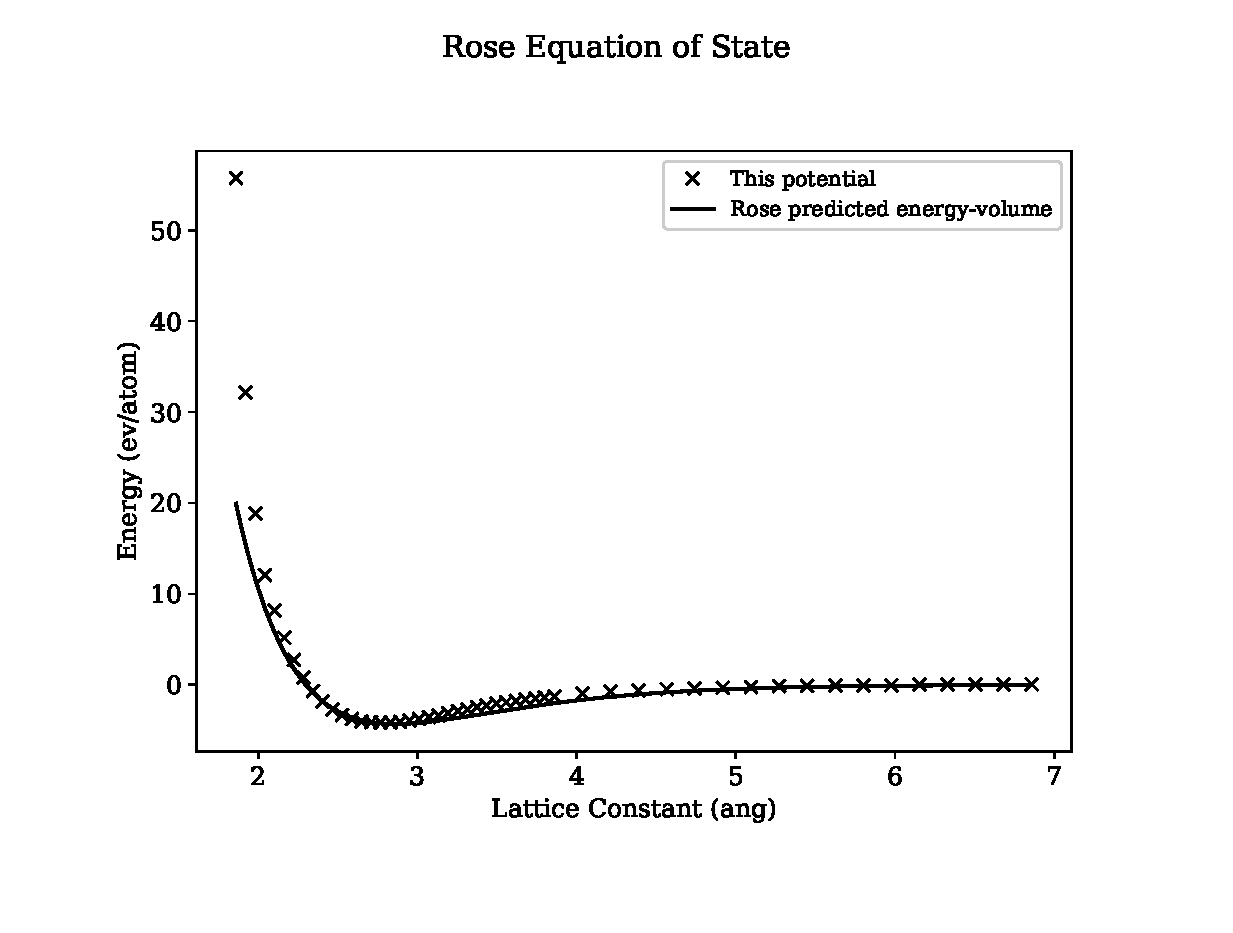
\includegraphics[width=.94\linewidth]{chapters/potentials_fe_pd_ru/fepd_potential/eos/rose_plot_bp_0.eps}  
  \caption{BCC Iron}
  \label{fig:sub-first}
\end{subfigure}
\begin{subfigure}{.32\textwidth}
  \centering
  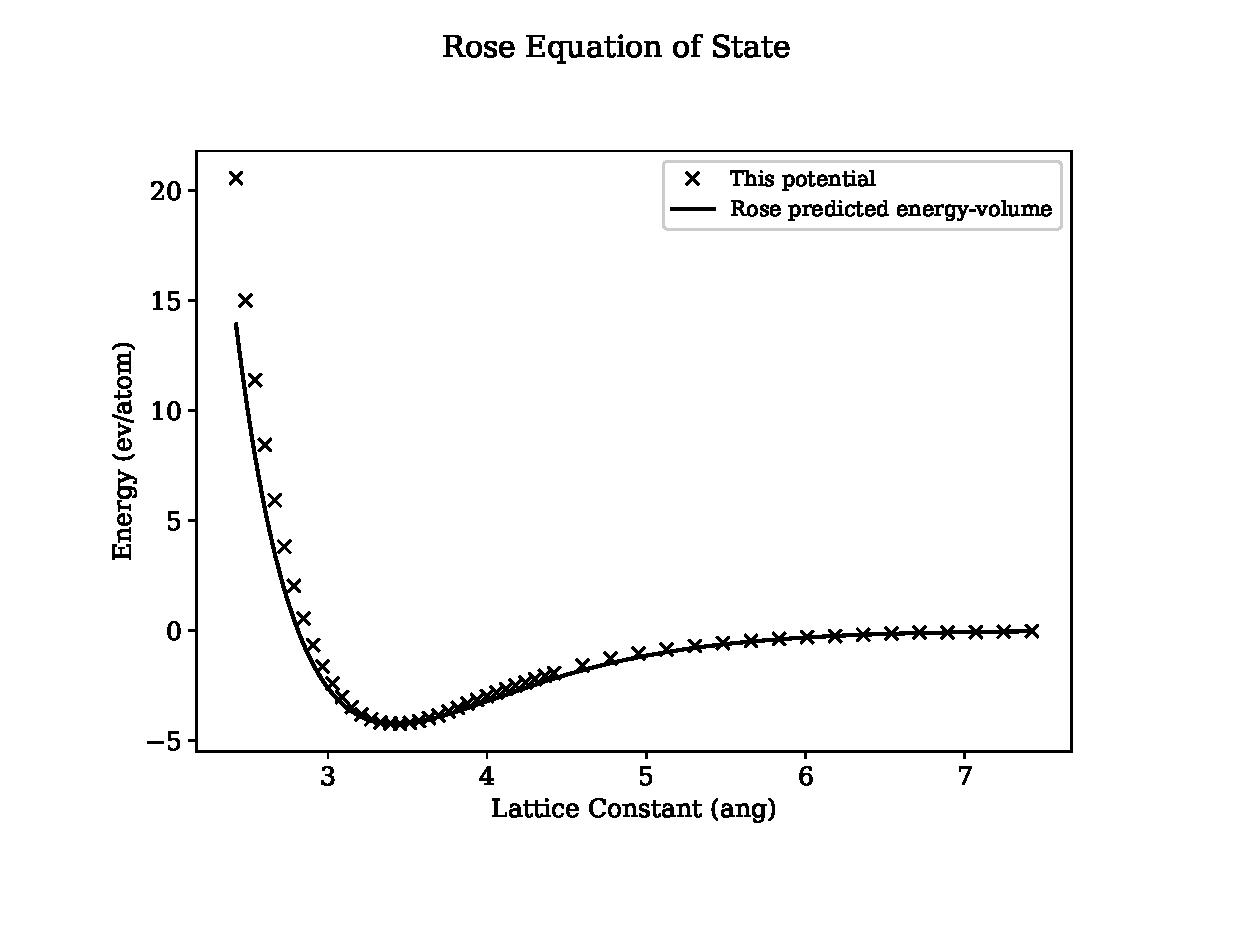
\includegraphics[width=.94\linewidth]{chapters/potentials_fe_pd_ru/fepd_potential/eos/rose_plot_bp_1.eps}  
  \caption{FCC Iron}
  \label{fig:sub-first}
\end{subfigure}
\label{fig:fe-rosevinet}
\caption{Rose-Vinet plots for Iron}
\end{figure}

Both the Birch-Murnaghan and Rose-Vinet equation of states were used to fit the potentials, and these are useful for fitting the bulk modulus (Birch-Murnaghan) and behaviour of the potential over a wider range of values for the lattice parameter (Rose-Vinet). The Rose-Vinet fit for Fe is given in figure \ref{fig:fe-rosevinet} for both the \acrshort{fcc} and \acrshort{bcc} structures.

\begin{figure}[htb]
\begin{subfigure}{.32\textwidth}
  \centering
  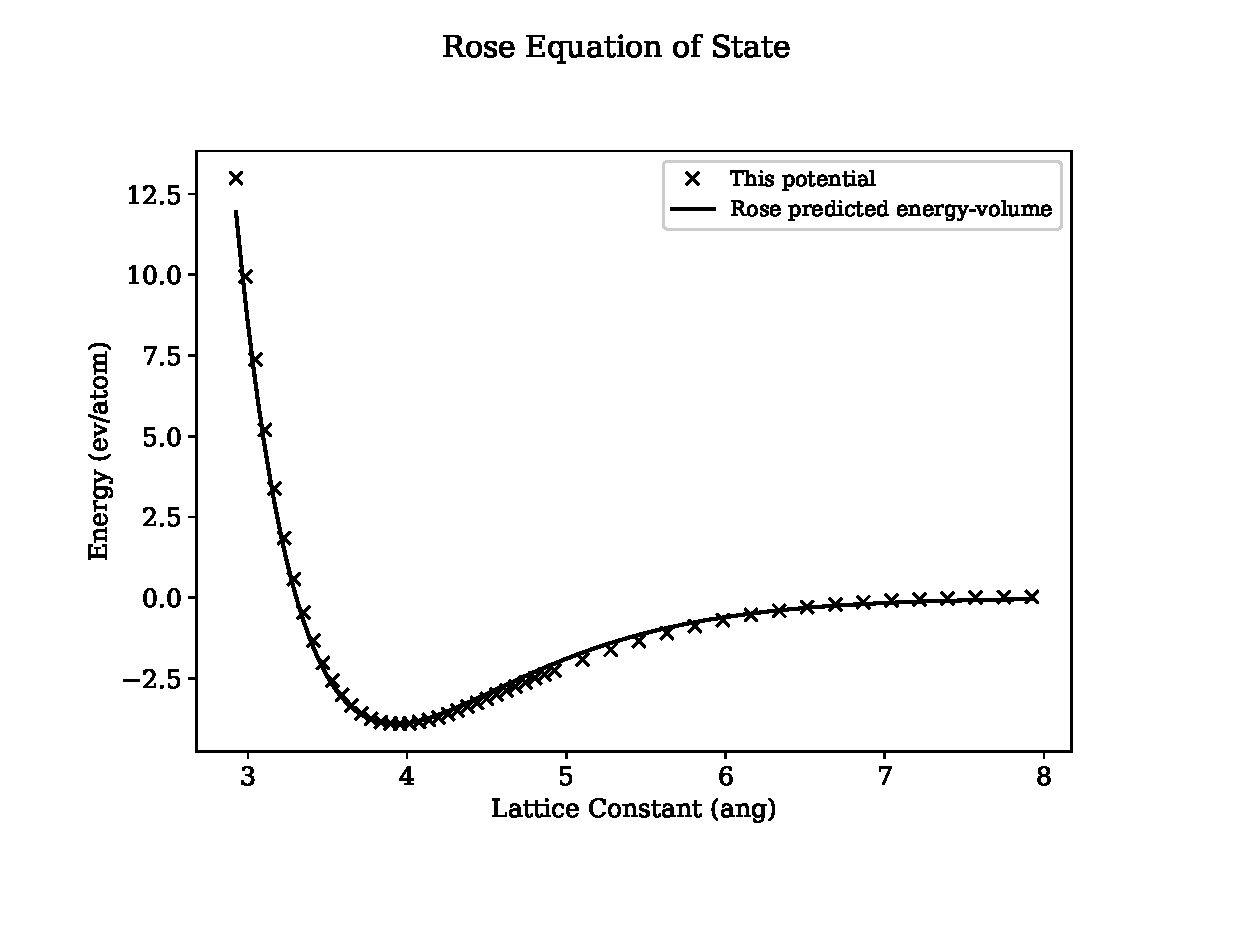
\includegraphics[width=.94\linewidth]{chapters/potentials_fe_pd_ru/fepd_potential/eos/rose_plot_bp_2.eps}  
  \caption{FCC Palladium}
  \label{fig:sub-first}
\end{subfigure}
\begin{subfigure}{.32\textwidth}
  \centering
  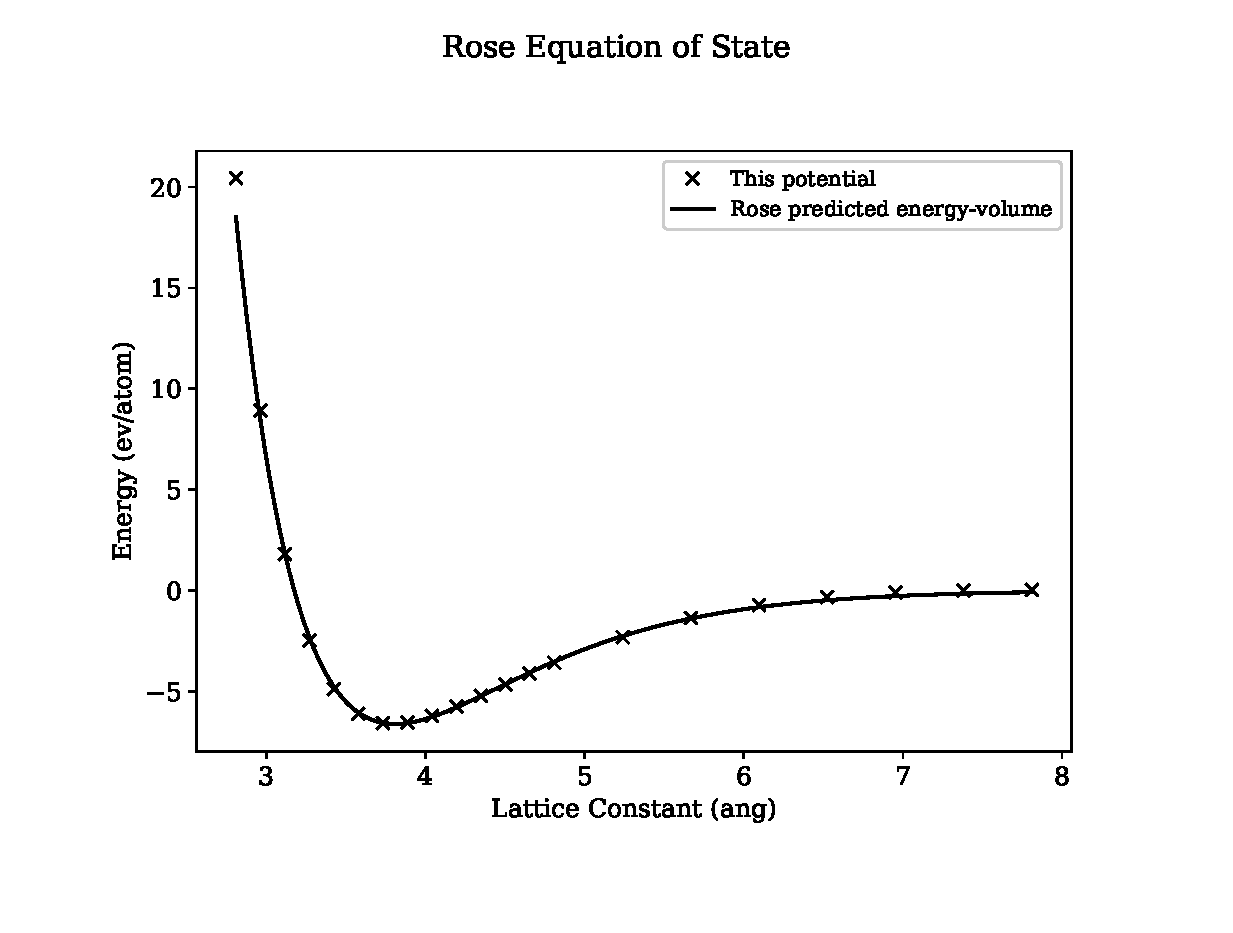
\includegraphics[width=.94\linewidth]{chapters/potentials_fe_pd_ru/feru_potential/eos/rose_plot_bp_2.eps}  
  \caption{FCC Ruthenium}
  \label{fig:sub-first}
\end{subfigure}
\label{fig:rupd-rosevinet}
\caption{Rose-Vinet plots for Palladium and Ruthenium}
\end{figure}

The Rose-Vinet fit for both Pd and Ru is given in figure \ref{fig:rupd-rosevinet} for just \acrshort{fcc} structures.  The potentials were then used to calculate the energies predicted by \acrshort{dft} and how well these fit, for both potentials, are given in figure \ref{fig:fepd-feru-fit}.

\begin{figure}[htb]
\begin{subfigure}{.32\textwidth}
  \centering
  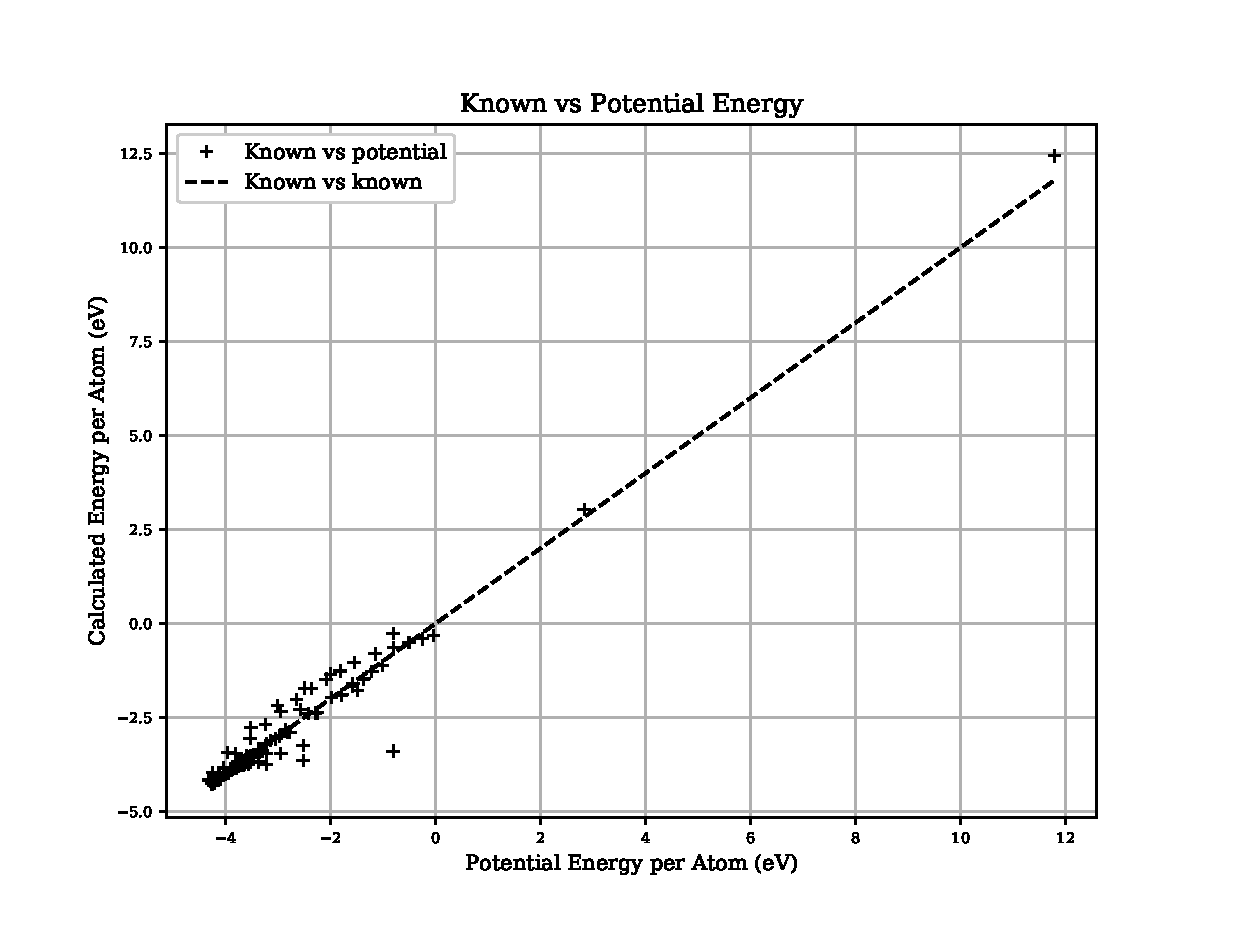
\includegraphics[width=.94\linewidth]{chapters/potentials_fe_pd_ru/fepd_potential/potential_known_energy_full_set.eps} 
  \caption{Fe-Pd}
  \label{fig:fepd-fit}
\end{subfigure}
\begin{subfigure}{.32\textwidth}
  \centering
  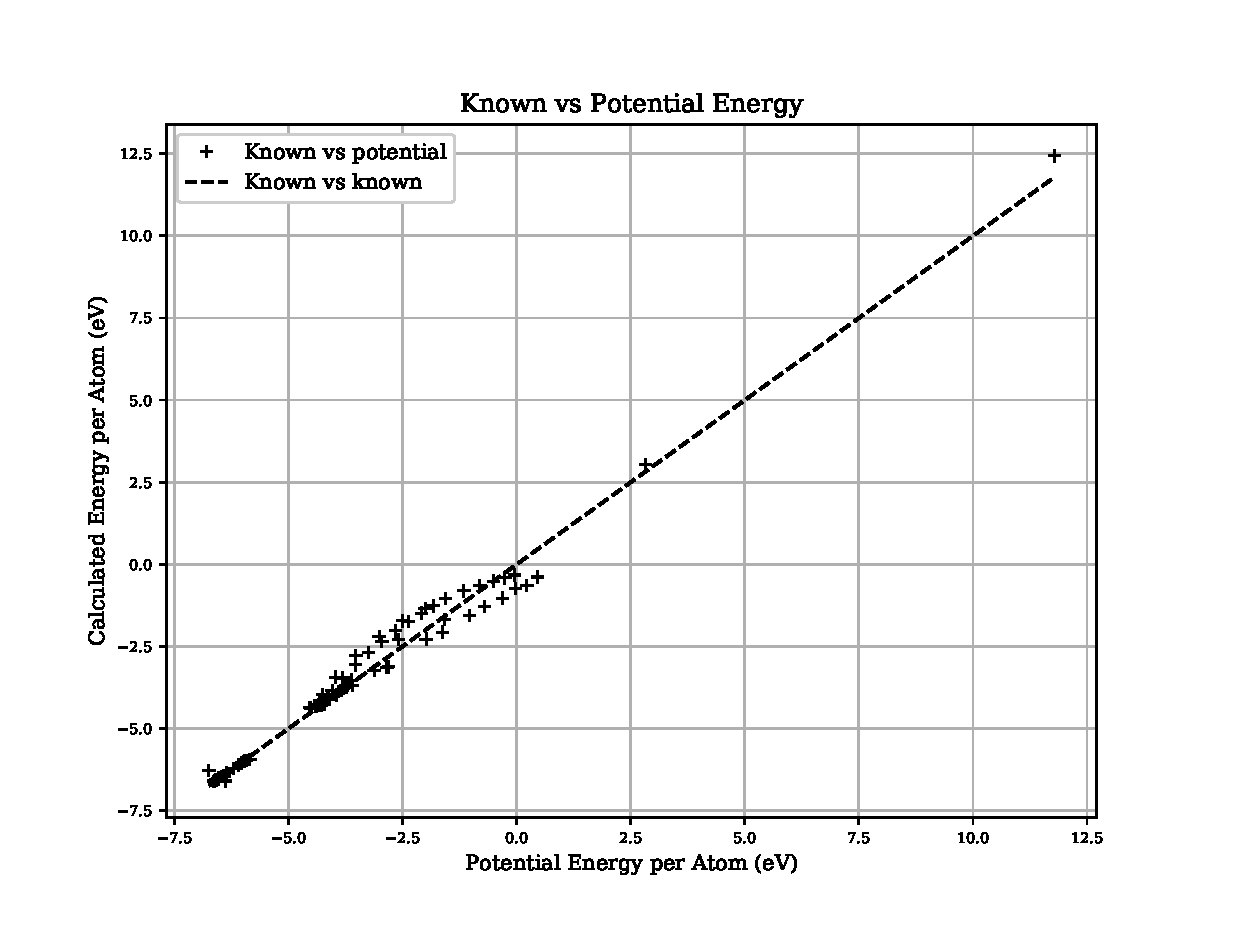
\includegraphics[width=.94\linewidth]{chapters/potentials_fe_pd_ru/feru_potential/potential_known_energy_full_set.eps} 
  \caption{Fe-Ru}
  \label{fig:feru-fit}
\end{subfigure}
\label{fig:fepd-feru-fit}
\caption{How well the potentials recreate \acrshort{dft} values}
\end{figure}

There has been very limited testing of the potentials with \acrshort{lammps} in order to verify that the output files are readable by the molecular dynamics code.  The code successfully reads in both potentials and was able to run a rudimentary simulation of Fe-Pd and Fe-Ru.  An single frame from a trial simulation of a 32,000 atom cube, made of 99\% Fe and 1\% Pd, is given in figure \ref{fig:fepd-lammps-trial}.

\begin{figure}[htb]
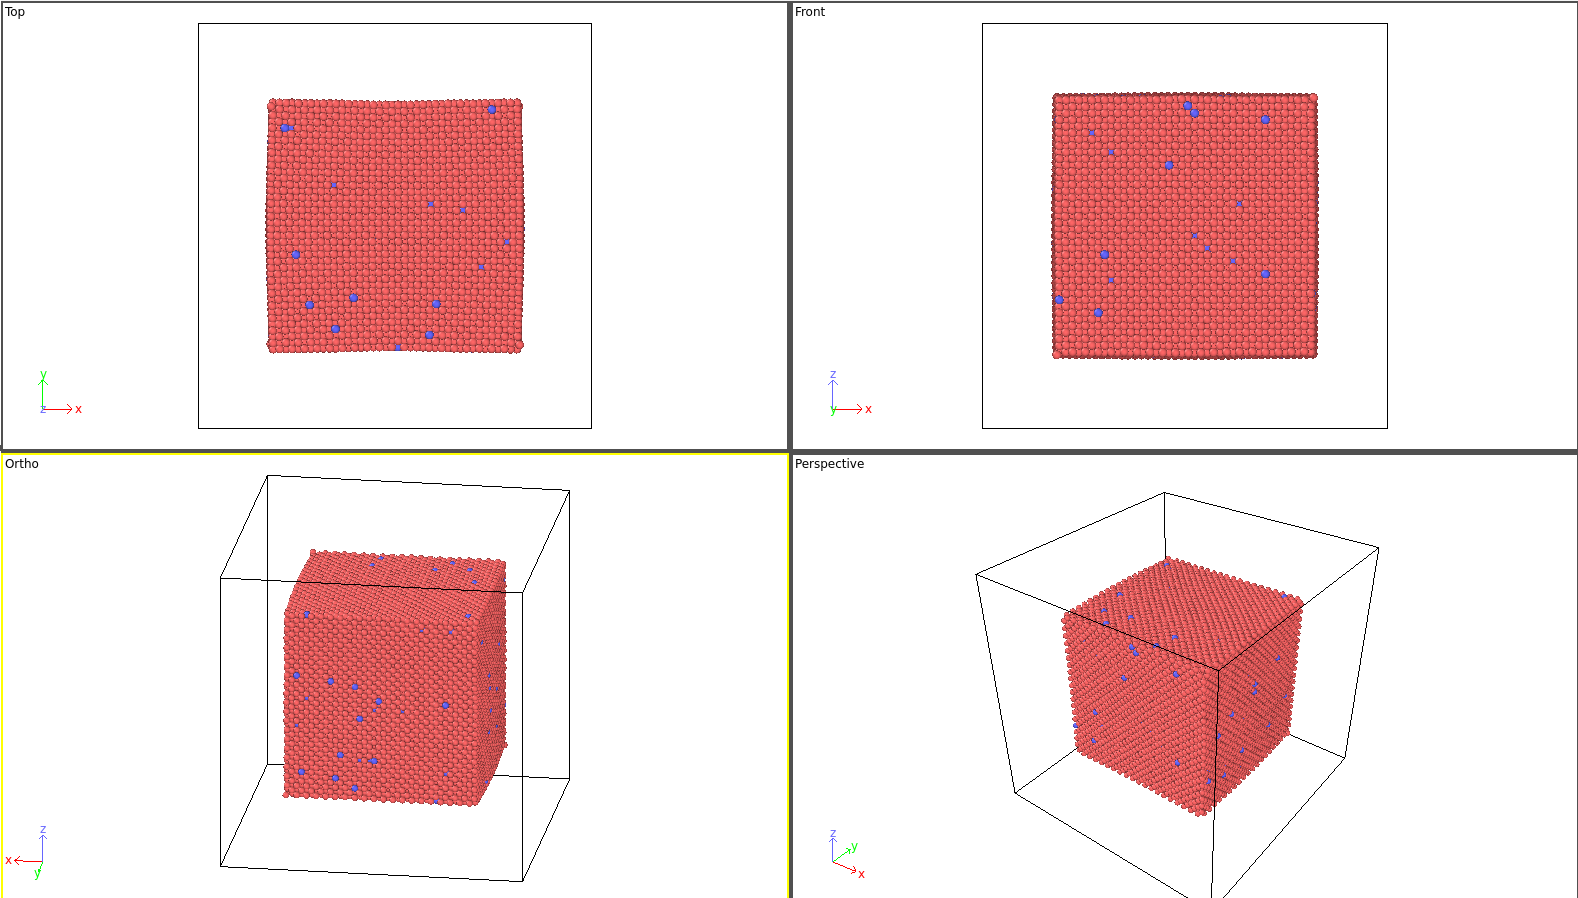
\includegraphics[width=.94\linewidth]{chapters/potentials_fe_pd_ru/lammps/fepd_fct_cube_particle.png} 
\label{fig:fepd-lammps-trial}
\caption{LAMMPS modelled cube like Fe-Pd particle}
\end{figure}

There is certainly room for improvement and this will be discussed in more detail in chapter \ref{chapter:conclusions}.  More data relating to the potentials is given in appendix \ref{chapter:appendix-fepdpotential} and \ref{chapter:appendix-ferupotential} and these detail the bulk properties of the potentials and compare how well they fit to the \acrshort{dft} computed values to which they are fit.



\section{DL\_POLY Contribution}

DL\_POLY is a Molecular Dynamics code developed by W. Smith, T.R. Forester and I.T. Todorov at Daresbury Laboratory in Warrington. It is written in Fortran and, before the modifications, included a number of potential types for metals including:

\begin{itemize}
\item Finnis Sinclair
\item EAM
\item EEAM
\end{itemize}

The Finnis Sinclair is a particular form of the EAM potential, and EEAM is a modification where, is the metal is an alloy, the density and embedding functional for each atom type are treated separately.

A meeting was held with Dr. Todorov at Daresbury Laboratory, where a brief overview of the relevant code was given.  After this point, and corresponding by email, the two band EAM type was added (2BEAM).  The code was altered with the addition of an array used to store the d-band density function and d-band embedding functional, with the s-band function/functional using the original density function and embedding functional arrays.  The calculation of energy and forces on atoms was also altered to make use of these arrays where a \acrlong{2beam} potential is used.

\begin{lstlisting}[style=sEmail,caption={DL\_POLY 4.05 mailshot extract}]
DL_POLY_4.05: New Release & Events - MAILSHOT 013

NEW FEATURES \& IMPROVEMENTS
--------------------------- 
1.  New two band (2B) EAM and EEAM potentials for metals (TEST45 and TEST46). 

Acknowledgements
----------------
Ben Palmer \@ University of Birmingham (UK) for contributing to the
development and testing of the 2BEAM for metals;

Regards,

Ilian Todorov
July 2013 


\end{lstlisting}

Extracts of the modified DL\_POLY code are included in appendix \ref{chapter:appendixdlpoly}.



